\chapter{Введение}

Введение по лекции от 7 сентября 2011 года, помнится была среда.

\section{Лектор}

{\large Куликов Александр Сергеевич}
\par\bigskip

e-mails (в порядке приоритета): \hfill kulikov@logic.pdmi.ras.ru 

\hfill alexander.s.kulikov@gmail.com
\par\bigskip

Дислокация в АФТУ: \hfill кабинет 412
\par\bigskip

\paragraph{Примечания:}

\begin{itemize}

\item В присутсии Омельченко А. В. обращаться по имени и отчесву.

\item Первый e-mail прикольнее, там символ @ очень удачно совпадает с именем.

\end{itemize}

\section{Литература}

Список литературы примерно следующий:

\begin{enumerate}
\item Algorithms. Авторы: S. Dasgupta, C. H. Papadimitriou, U. V. Vazirani (Ссылки: \url{http://www.cs.berkeley.edu/~vazirani/algorithms.html} или \url{http://www.mhhe.com/dasgupta})

\item Алгоритмы: построение и анализ. Авторы: Т. Кормен, Ч. Лайзерсон, Р. Ривест

\item Программирование: теоремы и задачи. Автор: А. Шень (Такой прикольный бородатый дядька)

\item Randomized Algorithms. Авторы: Rajeev Motwani, Prabhakar Raghavan.
\end{enumerate}

\section{Последовательность Фиббоначи}

\begin{equation}
	\begin{split}
		& F _0 = 0 \\
		& F _1 = 1 \\
		& F _n = F _{n-1} + F _{n-2}
	\end{split}
\end{equation}

Рост чисел Фиббоначи обычно оценивается следующей формулой:

\begin{equation}
	F _n = 2^{0.694 n}
	\label{math::fib_approx}
\end{equation}

Точное выражеие для n-ого числа фиббоначи называется формулой Бине:

\begin{equation}
	F _n = \frac{
		{\left (
			\frac{1 + \sqrt{5} } {2}
		\right )}^{n} - {
		\left (
			\frac{1 - \sqrt{5} } {2}
		\right )}^{n}
	}{\sqrt{5}}
\end{equation}

Теперь создадим простую программку определяющую n-ое число фиббоначи (здесь и в дальнейшем все программки будут написаны на Си или чем-то очень близком к нему, зависит от степени успевания за лекциями, желающим поучаствовать добро пожаловать, комментарии по стилю приветсвуются, а ругань нет).

\begin{lstlisting}
	unsigned long fib1(int n)
	{
		assert(n >= 0);

		if (n == 0) return 0;
		if (n == 1) return 1;
		return fib1(n-1)+fib1(n-2);
	}
\end{lstlisting}

Корректность приведенного вычисления вытекает из определения чисел фиббоначи, производительность же страдает страшно, для того, чтобы в этом убедится посмотрим на дерево рекурсии \ref{pic::rec_tree}, в котором явно видно, что вычисления, например, для n-2 повторяются два раза, для n-3 они повторяюся еще больше раз и так далее.

\begin{figure}[h]
	\noindent\center{
		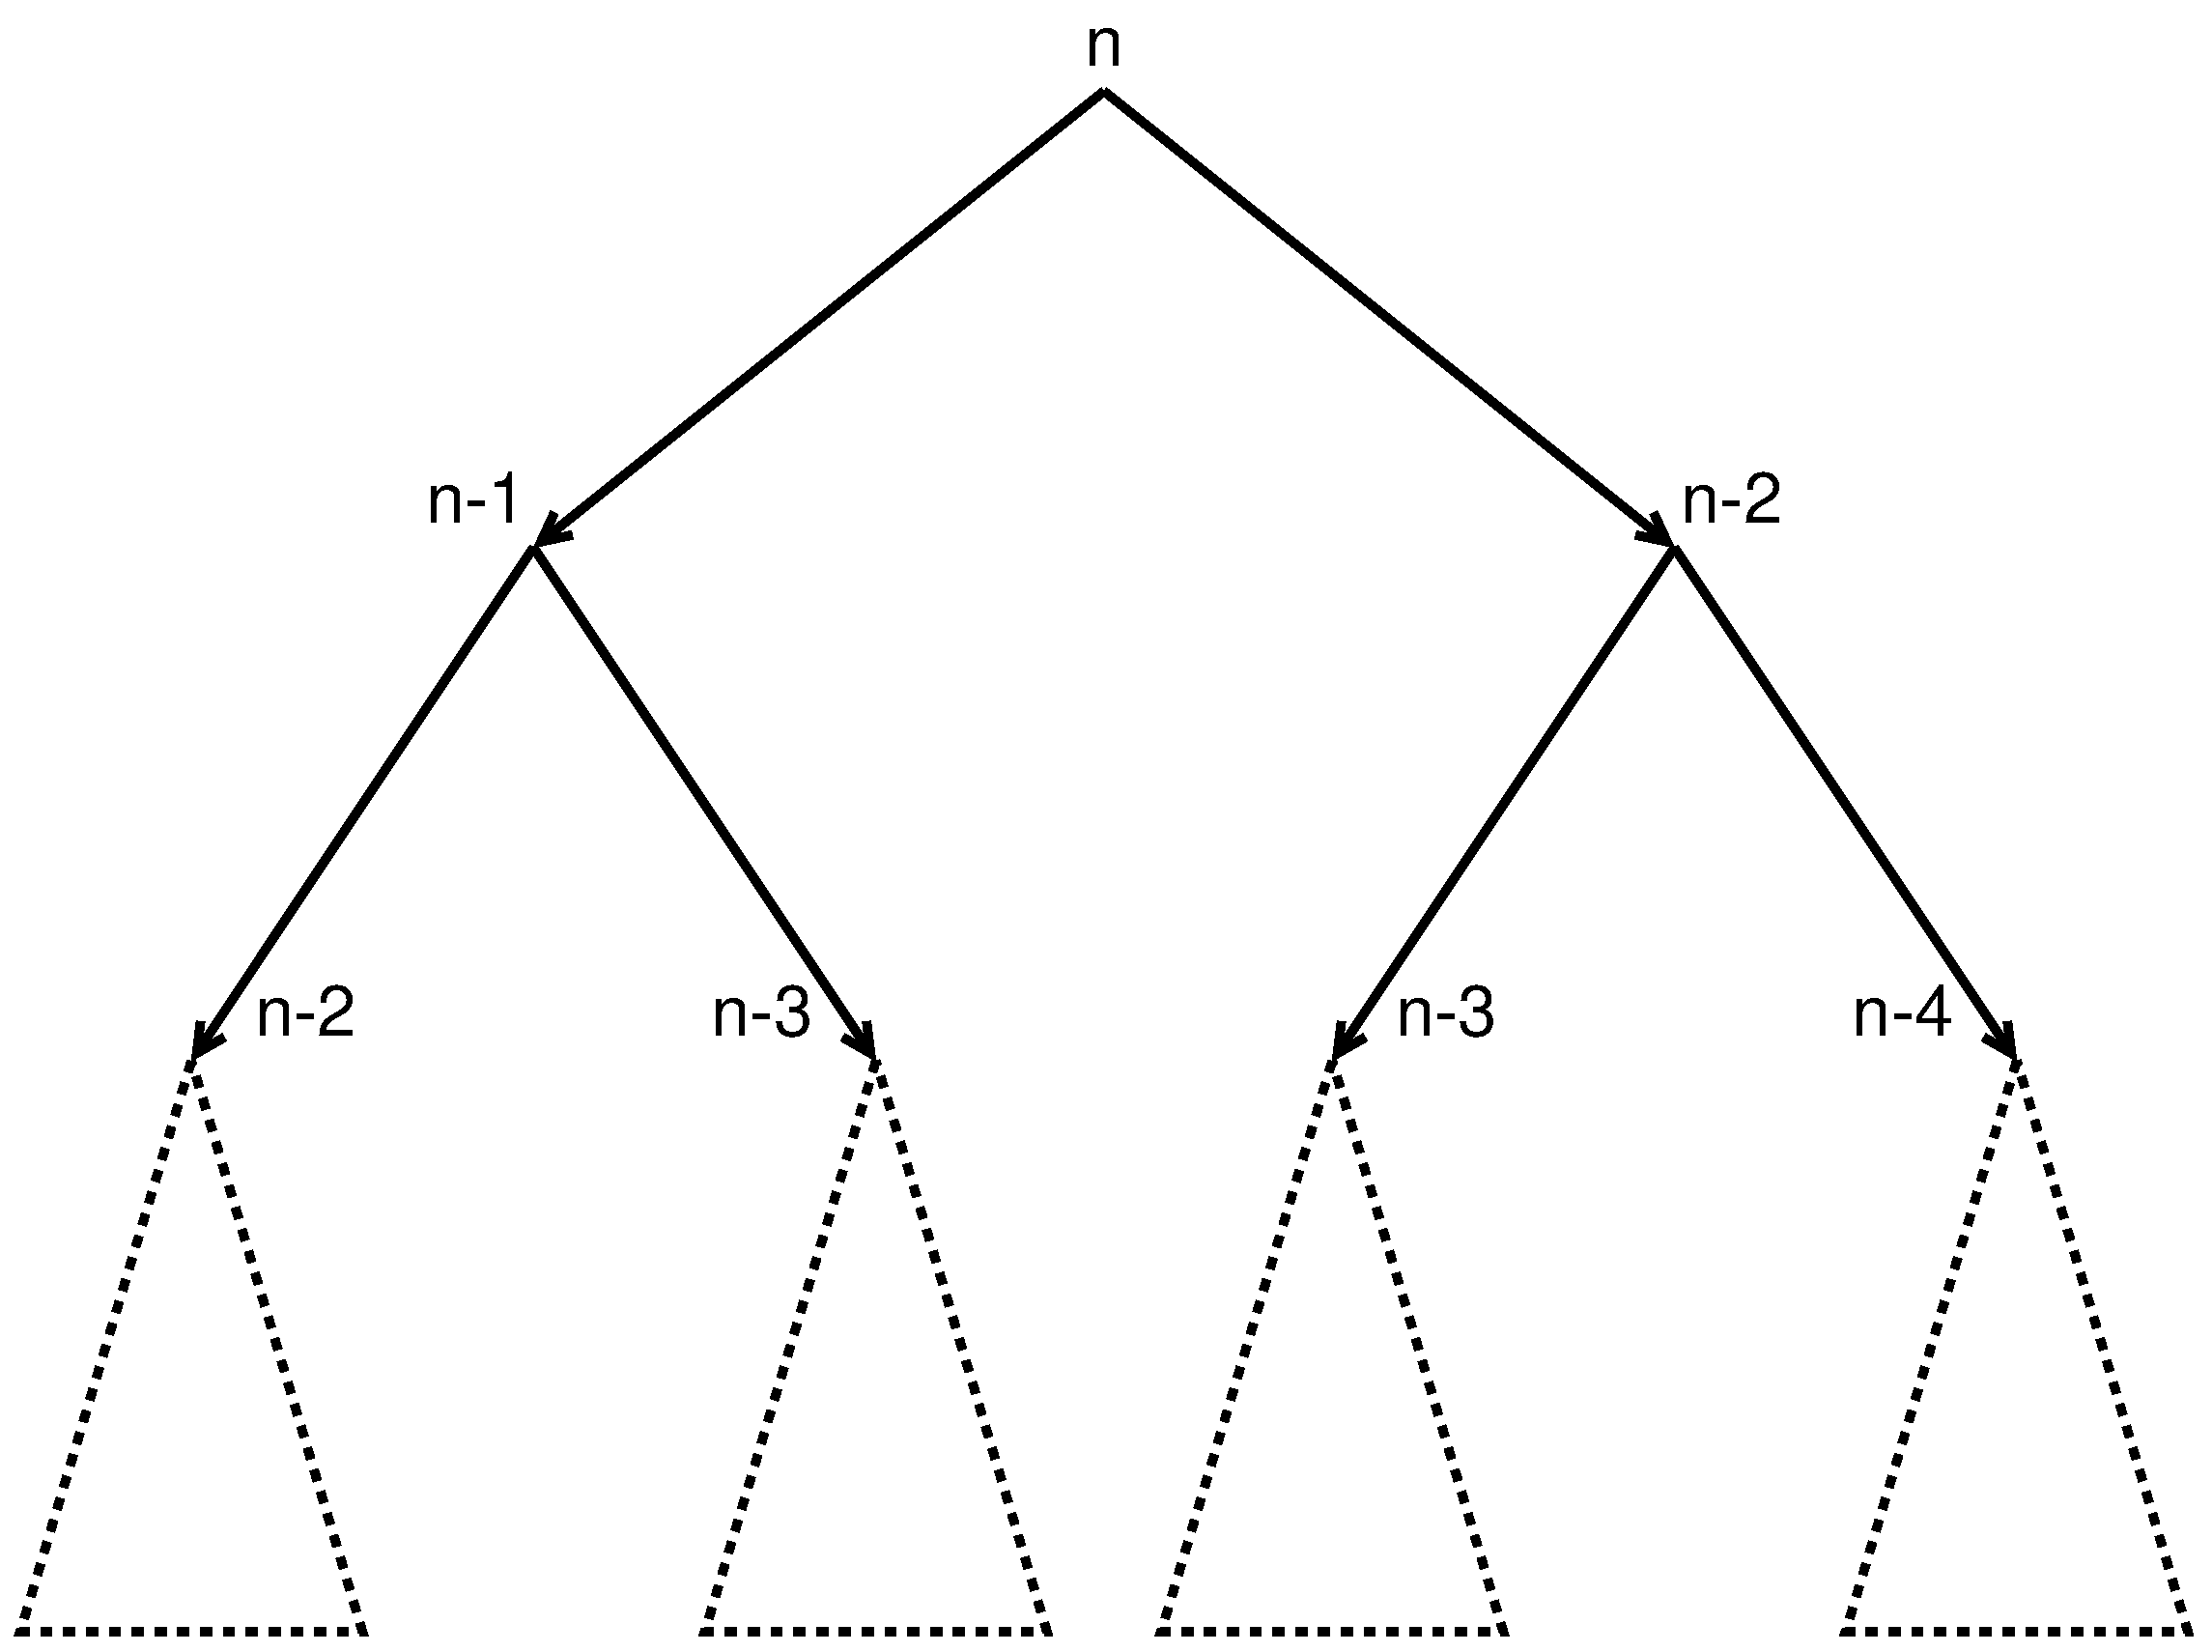
\includegraphics[width=0.5\linewidth]{fib1_tree}
	}
	\caption{Дерево рекурсии}
	\label{pic::rec_tree}
\end{figure}

Если достроить дерево до конца, то листья дерева будут содержать вызовы с параметрами 1 и 0, и в конечном итоге вычисление будет сводится к суммированию 0 и 1 (плюс расходы на рекурсивный вызов), таким образом временную сложность данного алгоритма можно оценить по следующей формуле:

\begin{equation}
	T \left ( n \right ) \approx C \cdot F _n
\end{equation}

Вообщем вычисление происходит очень неэффективно, попробуем улучшить наш алгоритм, для этого попытаемся избавится от повторных вычислений.

\begin{lstlisting}
	unsigned long fib2(int n)
	{
		unsigned long holder = 1, fib = 1, fnm1 = 0;

		assert(n >= 0);

		if (n == 0) return 0;
		if (n == 1) return 1;

		while(--n>0)
		{
			holder = fib;
			fib += fnm1;
			fnm1 = holder;
		}

		return fib;
	}
\end{lstlisting}

Данный алгоритм уже не пользуется рекурсивным спуском, а начинает вычислять число фиббоначи с первых элементов последовательности, ведь для получения нового числа фиббоначи, по определению, нужны лишь два предыдущих. Для доказательства корректности достаточно отметить, что внутри цикла до выполнения тела справедливо утверждение:

\begin{equation}
	\begin{split}
		& fib = F _i \\
		& holder = F _{i-1} = fnm1
	\end{split}
\end{equation}

а после:

\begin{equation}
	\begin{split}
		& fib = F _{i+1} \\
		& holder = F _i = fnm1
	\end{split}
\end{equation}

Таким образом получаем, что в переменной fib всегда содержится число фиббоначи, проверить, что это число с нужным номером не составляет труда.

Анализ временной сложности довольно очевиден, каждый элемент последовательности вычисляется всего один раз, а значит оценка временной сложности выражается следующей формулой:

\begin{equation}
	T \left ( n \right ) \approx C \cdot n
\end{equation}

Теперь небольшое лирическое отступление, получив линейную временную сложность в большинстве случаев можно было бы остановится, но давайте вспомним о том, что последовательность фиббоначи растет очень быстро (экспоненциально), а значит, уже через небольшое время числа фиббоначи перестанут помещаться в размер стандартных целых чисел, представим теперь, что нам необходимо узнать число фиббоначи с очень большим номером, что делать в этом случае? В данном случае поможет длинная арифметика.

Для вычисления чисел фиббоначи требуется только операция сложения (ну и копирования, но пока оставим это в стороне), сложность операции сложения двух длинных целых чисел зависит от их разрядности (которая зависит от используемого основания BASE), но в целом можно сказать, что в лучшем случае (когда не было никаких переносов через разряды) сложение займет ровно столько операций, сколько разрядов в числе.

Давайте рассмотрим основание $ BASE = 2 $, тогда можно очень удобно воспользоваться оценкой для нахождения количества бит n-ого числа фиббоначи $ l = 0.694n $, и в таком случае оценка порядка роста алгоритма преобразовывается:

\begin{equation}
	T \left ( n \right ) > C \cdot n^2
\end{equation}

Таким образом можно увидеть, что смена базовой операции очень попортила оценку.

\section{Нотации}

При анализе алгоритмов приянто рассматривать не его сложность, а порядок роста сложности, т. е. анализировать как изменится время (затрачиваемая память и тд), при увеличении объема входных данных. Для описания порядка роста используются следующие обозначения:

\begin{Def}
	\label{def::o_notation}
	Говорят, что $ f = O ( g ) $, если существует такие положительные числа $ n _0 $ и $ C $, что для любого $ n > n _0 $ справедливо утверждение, что $ f ( n ) \le g ( n ) $ 

	$ \left [ f = O ( g ) \right ] \Leftrightarrow \left [ \exists ( c > 0 , n _0 > 0) : \forall ( n > n _0 ) f ( n ) \le C \cdot g ( n ) \right ] $
\end{Def}

\begin{Def}
	\label{def::omega_notation}
	Говорят, что $ f = \Omega ( g ) $, если существует такие положительные числа $ n _0 $ и $ C $, что для любого $ n > n _0 $ справедливо утверждение, что $ f ( n ) \ge g ( n ) $ 

	$ \left [ f = \Omega ( g ) \right ] \Leftrightarrow \left [ \exists ( c > 0 , n _0 > 0) : \forall ( n > n _0 ) f ( n ) \ge C \cdot g ( n ) \right ] $
\end{Def}

\begin{Def}
	\label{def::theta_notation}
	Говорят, что $ f = \Theta ( g ) $, если одновременно $ f = O ( g ) $ и $ f = \Omega ( g ) $

	$ \left [ f = \Theta ( g ) \right ] \Leftrightarrow \left [ f = O ( g ) \bigwedge f = \Omega ( g ) \right ] $
\end{Def}

Для работы с данной системой обозначений достаточно запомнить небольшой набор простых "правил":

\begin{itemize}
\item Мультипликативные и адитивные константы в выражениях можно отбрасывать

\item $ n^a $ растет не медленнее $ n^b $ при $ a \ge b $

\item Полиномиальная функция растет медленнее экспонециальной

\item Степень логарифма растет медленнее полиномиальной функции
\end{itemize}

\paragraph{Примеры}

Все примеры достаточно простые (местами тупые), просто чтобы все втянулись:

$ n^3 = \Omega ( n^2 ) $

$ n^2 = \Omega ( n \log ^5 n ) $

$ 3n \log n = O ( n^2 ) $

$ 7n^2 + 2n - 2 = \Theta ( n^2 ) $

$ n-200 = \Theta ( n - 100 ) $

\paragraph{Примечание}

На практике говорить только о порядке роста алгоритма не совсем верно, для того чтобы понять это рассмотрим пары функций:
\par\bigskip

\hbox to 0.6\linewidth {$ 1.001^n $ \hfill $ n^{5000} $}
\par\bigskip

\hbox to 0.6\linewidth {$ 1000n^3 + 50n^2 -200 $ \hfill $ \frac{1}{3}n^3 - n^2 - n $}

В общем заключаю, что на практике, иногда, величина $ n_0 $ из определений \ref{def::o_notation} и \ref{def::omega_notation} может быть настолько большой, что функция с большим порядком роста окажется лучше, хотя такое, наверно, встречается не слишком часто.

\section{Упражнения}

(Упражнения взяты из Algorithms. Авторы: S. Dasgupta, C. H. Papadimitriou, U. V. Vazirani, глава называется Prologue)

\textit{Упражнение 1. Определить в каких отношениях находятся функции f и g, $ f = O ( g ) $, $ f = \Theta ( g ) $ или $ f = \Omega ( g ) $}
\begin{enumerate}
\item $ n-100 $ и $ n - 200 $. Ответ: $ n-100 = \Theta ( n-200 ) $

\item $ n^{\frac{1}{2}} $ и $ n^{\frac{2}{3}} $. Ответ: $ n^{\frac{1}{2}} = O ( n^{\frac{2}{3}} ) $

\item $ 100n + \log n $ и $ n + \log ^2 n $. Ответ: $ 100n + \log n = \Theta ( n + \log ^2 n ) $

\item $ n \log n $ и $ 10n \log 10n $. Ответ: $ n \log n = \Theta ( 10n \log 10n ) $ 

\item $ \log 2n $ и $ \log 3n $. Ответ: $ \log 2n = \Theta ( \log 3n ) $

\item $ 10 \log n $ и $ \log n^2 $. Ответ: $ 10 \log n = \Theta ( \log n^2 ) $ (Преобразование: $ \log n^2 = 2 \log n $)

\item $ n^{1.01} $ и $ n \log ^2 n $. Ответ: $ n^{1.01} = \Omega ( n \log ^2 n ) $

\item $ \frac{n^2}{\log n} $ и $ n (\log n)^2 $. Ответ: $ \frac{n^2}{\log n} = \Omega ( n (\log n)^2 ) $ (Примечание: сокращаем $ n $ и домножаем на $ \log n $)

\item $ n^{0.1} $ и $ \log ^{10} n $. Ответ: $ n^{0.1} = \Omega ( \log ^{10} n ) $

\item $ \log ^{\log n} n $ и $ \frac{n}{\log n} $. Ответ: $ \log ^{\log n} n = \Omega ( \frac{n}{\log n} ) $ (Примечание: домножаем все на $ \log n $, дальше применяем к левой и правой части $ \log _{\log _n} $ и сравниваем основания полученных логарифмов, в одном константа, в другом возрастающая варианта)

\item $ \sqrt{n} $ и $ \log ^3 n $. Ответ: $ \sqrt{n} = \Omega ( \log ^3 n ) $ (Примечание: слева полином, справа логарифм, просто по правилу)

\item $ n^{\frac{1}{2}} $ и $ 5^{\log _2 n} $. Ответ: $ n^{\frac{1}{2}} = O ( 5^{\log _2 n} ) $ (Примечание: $ n^{\frac{1}{2}} = 5^{\log _5 \sqrt{n}} = 5^{C \log _2 n} $ причем $ C < 1 $)

\item $ n2^n $ и $ 3^n $. Ответ: $ n2^n = O ( 3^n ) $ (Примечние: поделите одно на другое)

\item $ 2^n $ и $ 2^{n+1} $. Ответ: $ 2^n  = \Theta ( 2^{n+1} ) $ (Преобразование: $ 2^{n+1} = 2 \cdot 2^{n} $)

\item $ n! $ и $ 2^n $. Ответ: $ n! = \Omega ( 2^n ) $ (Примечание: по формуле Стирлинга $ n! \approx \sqrt{2 \pi n} \left ( \frac{n}{e} \right )^n $)

\item $ (\log n) ^ {\log n} $ и $ 2^{(\log _2 n)^2} $. Ответ: $ (\log n) ^ {\log n} = O ( 2^{(\log _2 n)^2} ) $ (Примечание: $ 2^{(\log _2 n)^2} = 2^{\log _2 n \cdot \log _2 n} = n^{\log _2 n} $)

\item $ \Sigma ^n _{i=1} i^k $ и $ n^{k+1} $. Ответ: $ \Sigma ^n _{i=1} i^k = \Theta ( n^{k+1} ) $ (Примечание: раскрываем правую часть $ n^{k+1} = n \cdot n^{k} = \Sigma ^n _{i=1} n^k $ и сразу станоится понятно, почему выполняется O, но кроме этого справедливо $\sum^{n}_{i=1} i^k \ge n \frac{n}{2}^k$)
\end{enumerate}

\textit{Упражнение 2. Покажите что, если $ C $ положительное число, тогда $ g(n) = 1 + c + c^2 + ... + c^n $}

\begin{enumerate}
\item $ \Theta ( 1 ) $ при $ С < 1 $. Доказательство: если $ C \ne 1 $, тогда $ g(n) = \frac{1 - C^{n+1}}{1 - C} < \frac{1}{1 - C} $

\item $ \Theta (n) $ при $ С = 1 $. Доказательство: ну блин, ну вы поняли...

\item $ \Theta (C^n) $ при $ C > 1 $. Доказательство: опять же $ g(n) = \frac{1 - C^{n+1}}{1 - C} $
\end{enumerate}

\textit{Упражнение 3. Задачи на оценку скорости роста чисел фиббоначи}

\begin{enumerate}
\item Доказать, что $ F _n \ge 2^{0.5n} $ при $ n \ge 6 $. Доказательство: пусть условие выполняется для $ n = 6 $ и $ n = 7 $ (это действительно так), тогда предположим, что условие истинно для $ F _n $ и $ F _{n+1} $ (как раз наши 6 и 7), тогда имеем следующее $ F _{n+2} = F _n + F _{n+1} \ge 2^{\frac{n}{2}} + 2^{\frac{n+1}{2}} > 2 \cdot 2^{\frac{n}{2}} = 2^{\frac{n+2}{2}} $

\item Найти константу $ С < 1 $ такую, что $ F _n \le 2^{cn} $ для всех $ n \ge 0 $, и показать, что результат корректен. Ответ: $ C = - \log \frac{-1 + \sqrt{5}}{2} \approx 0.694241914 $ (Решение: $ F _n = F _{n-1} + F _{n-2} < 2^{C(n-1)} + 2^{C(n-2)} \le 2^{Cn} \Leftrightarrow 2^{-C} + 2^{-2C} \le 1$, далее делаем замену и решаем квадратное уравнение)

\item Найти наибольшую $ C $ такую, что $ F _n = \Omega ( 2^{Cn} ) $. Ответ: мне кажется, что это константа из предыдущего ответа, но надо это аккуратно доказать.
\end{enumerate}

\textit{Упражнение 4. Как посчитать числа фиббоначи быстрее}

Для этого воспользуемся следующим соображением:

\begin{equation}
	{\begin{pmatrix}
		1 & 1 \\
		1 & 0 \\
	\end{pmatrix}} ^ n =
	\begin{pmatrix}
		F _{n+1} & F _n \\
		F _n & F _{n-1} \\
	\end{pmatrix}
	\label{math::fib_matrix}
\end{equation}

Самым примитивным способом перемножение двух матриц занимает 4 сложения и 8 умножений (но кроме этого алгоритма существуют еще и алгоритмы быстрого перемножения матриц, например, алгоритм Штрассена, который позволяет уменьшить число перемножений за счет большего числа сложений), кроме того, матрица очевидно симметрична, а значит достаточно 6 произведений и 3 сложения.

Далее вспомним еще и алгоритм быстрого возведения в степень (способ очень похожий на схему горнера), выражаю общую идею алгоритма. Пусть $ n = ( n_k, n_{k-1}, ... , 0 )$ - двоичное представление показателя степени, тогда число $ x ^ n $ может быть представлено следующим образом:

\begin{multline}
	x^n = x ^{
		\left (
			\left (
				...
				\left (
					\left ( 
						n_k \cdot 2 + n_{k-1}
					\right )
					\cdot 2 + n_{k-2}
				\right )
				\cdot 2 + ...
			\right )
			\cdot 2 + n_1
		\right )
		\cdot 2 + n_0 } = \\ =
		{\left (
			...
			{\left (
				{\left (
					{\left (
						x^{n_k}
					\right )
					}^2 \cdot x^{n_{k-1}}
				\right )
				}^2 ...
			\right )
			}^2 \cdot x^{n_1}
		\right )
		}^2 \cdot x^{n_0}
\end{multline}

Далее, чтобы развернуть число согласно машинному представлению мы вносим двойки в показателях степеней внутрь скобок (при внесении, естественно, показатели перемножаем) и получаем следующее соотношение:

\begin{equation}
	x^n = \Pi ^{k} _{i=0} x^{n_i^{(2^{i})}}
\end{equation}

На СИ это будет выглядеть следующим образом:

\begin{lstlisting}
	long int qpow(int number, unsigned int power)
	{
		int res = 1, temp = number;

		while (power) {
			if (power % 2) res *= temp;
			if (power >>= 1) temp *= temp;
		}

		return res;
	}
\end{lstlisting}

Таким образом количество перемножений матриц, требуемое при таком алгоритме, зависит от числа нулевых и единичных бит в двоичном представлении показателя степени, и, очевидно, пропорционально числу бит требуемых для представления показателя степени, т. е. возведение матрицы в степень требует следующего числа перемножений матриц:

\begin{equation}
	T(n) = \Theta ( \log _2 n )
\end{equation}

Теперь получается, что если для вычисления $F_n$ требуется возвести матрицу \ref{math::fib_matrix} в n-1 степень, получаем логарифмическую сложность (по количеству умножений), теперь пусть операция умножения двух n-битных чисел требует $O (M(n))$ битовых операций, кроме того не трудно увидеть, что все промежуточные результаты перемножений не могут быть больше чем число $F_n$, т. к. также являются числами фиббоначи с меньшим номером, и учитывая соотношение \ref{math::fib_approx}, получаем сложность нахождения числа фиббоначи по числу битовых операций:

\begin{equation}
	T(n) = O (M(n) \log n)
\end{equation}

Для "школьного" алгоритма перемножения чисел $M(n) = O (n^2)$, что не очень хорошо. Но теперь давайте прекинем, что количество бит в числах вообще говоря растет постепенно, и можно даже сказать больше, что с каждым разрядом степени, в которую мы возводим матрицу, число бит в представлении числа удваивается (разряд степени или умножение показателя степени на 2 эквиваленто возведению имеющейся матрицы в квадрат, в этом случае, если $O(2^{n})$ оценка числа фиббоначи в матрице, то $2^{(n^2)}$ оценка числа фиббоначи в матрице возведенной в квадрат, далее для количества бит в пером числе справедлива оценка $O(\log {2^n}) = O (n)$, а для количества бит во втором числе $O (\log {2^{(n^2)}}) = O (\log {n^2}) = O (2 \log n)$ т. е. удваивается), тогда можно сказать, что общее число битовых операций :

\begin{equation}
	T(n) = O \left( \sum_{i=0}^{\lceil \log n \rceil} M(2^i) \le M \left(\sum_{i=0}^{\lceil \log n \rceil} 2^i \right) \right) = O \left( M \left( n \right) \right)
\end{equation}

\paragraph{Замечание} Предыдущее преобразование возможно пожалуй только для выпуклых функций (см. неравенство Йенсена)

Таким образом эффективность третьего алгоритма вычисления чисел фиббоначи зависит от эффективности перемножения двух битовых чисел. И для получения ускорения необходим алгоритм работы работающий быстрее чем $O (n^2)$

\section{Post scriptum}

PS: я знаю, что правильно писать Фибоначчи.

PPS: все баги это не баги а фичи, но опечатки все-таки постараемся исправить.

PPPS: продолжение следует
